\documentclass[11pt]{article}

\usepackage[a4paper,margin=1in]{geometry}
\usepackage[T1]{fontenc}
\usepackage[utf8]{inputenc}
\usepackage{lmodern}
\usepackage{microtype}
\usepackage{amsmath,amssymb,amsthm,mathtools}
\usepackage{booktabs}
\usepackage{array}
\usepackage{multirow}
\usepackage{graphicx}
\usepackage{algorithm}
\usepackage{algpseudocode}
\usepackage{enumitem}
\usepackage{xcolor}
\usepackage{hyperref}
\usepackage{pgfplots}
\pgfplotsset{compat=1.18}

\hypersetup{
  colorlinks=true,
  linkcolor=blue!55!black,
  citecolor=blue!55!black,
  urlcolor=blue!55!black
}

\newtheorem{definition}{Definition}
\newtheorem{lemma}{Lemma}
\newtheorem{theorem}{Theorem}
\newtheorem{problem}{Problem}
\newtheorem{proposition}{Proposition}

\newcommand{\supp}{\operatorname{supp}}
\newcommand{\aocc}{\operatorname{aocc}}
\newcommand{\socc}{\operatorname{socc}}
\newcommand{\cl}{\operatorname{cl}}
\newcommand{\Env}{\operatorname{Env}}
\newcommand{\EnvR}{\operatorname{Env}_{R}}
\newcommand{\Hraw}{\mathcal{H}_{\mathrm{raw}}}
\newcommand{\Hclosed}{\mathcal{H}_{\mathrm{closed}}}

\title{AURA-HOI: Auditable Unified Representative Mining for High-Occupancy Itemsets}
\author{Minh Quan Van Ha\\Independent Researcher}
\date{}

\begin{document}
\maketitle

\begin{abstract}
High-occupancy itemset mining (HOIM) extends classical support-based itemset mining by requiring an itemset to occupy a large fraction of the transactions in which it appears. This density-oriented objective is useful when support alone is insufficient: an itemset may appear frequently while still representing only a small portion of each supporting transaction. However, occupancy is not anti-monotone under itemset extension, so the pruning principles used by Apriori-style frequent itemset mining cannot be transferred directly. Existing HOI miners also differ in output semantics: some enumerate threshold-complete raw itemsets, whereas others return top-$k$, maximal, adaptive-threshold, or closed representatives. This paper proposes AURA-HOI, an auditable high-occupancy itemset mining algorithm that separates the mathematical scoring semantics from the reported output view. AURA-HOI provides a raw fullset mode for direct equality comparison with HEP and DFHOI, and a support-class representative mode for compact closed-output analysis. The method combines vertical bitset evidence, residual occupancy-envelope pruning, support-closure certificates, and summed-occupancy compatibility for repository-level baseline matching. On Mushrooms at $\alpha=0.10$, AURA-HOI returns the same 955 raw HOIs as HEP and DFHOI while reducing runtime from 2.256 seconds to 1.262 seconds against HEP and reducing peak memory from 890.74 MB to 3.77 MB. These results indicate that AURA-HOI can preserve exact raw-output semantics while providing a cleaner audit layer for comparing raw, closed, and representative HOI views.
\end{abstract}

\noindent\textbf{Keywords:} high-occupancy itemset mining; frequent itemset mining; closed itemsets; vertical bitsets; support equivalence; output normalization; occupancy pruning; reproducible pattern mining.

\section{Introduction}
Pattern mining studies the discovery of meaningful combinations of items from transactional data. In classical association-rule mining, the computational core is frequent itemset mining: rules are derived after finding itemsets whose supports exceed a user-defined threshold \cite{agrawal1993mining,agrawal1994fast}. The success of frequent itemset mining is strongly tied to the anti-monotonicity of support. If an itemset is infrequent, then all of its supersets are also infrequent. This simple property enables level-wise pruning in Apriori \cite{agrawal1994fast}, compressed pattern-growth in FP-growth \cite{han2000mining}, and efficient transaction-id intersections in vertical methods such as Eclat \cite{zaki2000scalable}.

Support, however, measures only how many transactions contain an itemset. It does not measure how much of those transactions the itemset explains. In a long transaction, a small itemset may be present but still occupy only a minor fraction of the transaction. This distinction motivated high-occupancy itemset mining (HOIM), where the interestingness of an itemset depends on its occupancy contribution $|X|/|t|$ inside the transactions that contain it \cite{deng2020mining}. Deng's original HOI formulation introduced the HEP algorithm, occupancy-list structures, and an upper-bound strategy for pruning the non-anti-monotone occupancy search space \cite{deng2020mining}. Later work improved HOI mining with equivalence classes, early pruning, incremental pattern mining, and top-$k$ variants \cite{nguyen2023efficient,kim2022mining,yildirim2025topk}.

Despite these advances, HOI mining remains difficult to compare scientifically. The difficulty is not only runtime. Different implementations may return different pattern families. A raw HOI miner enumerates every itemset satisfying a threshold. A top-$k$ miner returns only the highest-ranked patterns. A maximal miner compresses output by removing non-maximal patterns. A closed miner emits support-equivalence representatives rather than all raw itemsets. These views are useful for different purposes, but their itemset counts cannot be compared directly. A smaller output may reflect better compression rather than equivalent mining under the same semantics.

This paper proposes AURA-HOI (Auditable Unified Representative Algorithm for HOI), an HOI-only algorithm designed to make output semantics explicit. AURA-HOI treats raw itemsets, closed representatives, and top-$k$ representatives as views over a common occupancy foundation. Its raw mode supports direct equality comparison with HEP and DFHOI under summed-occupancy compatibility. Its closed mode stores support-class certificates, so each representative can be related back to a support-equivalence class. The objective is not merely to make another fast miner, but to make HOI comparisons auditable.

The contributions are as follows.
\begin{enumerate}[leftmargin=*]
  \item \textbf{Unified output semantics.} The paper formalizes raw HOI output, summed-occupancy compatibility, support-closed representatives, and support-class certificates in one framework.
  \item \textbf{Residual occupancy-envelope pruning.} AURA-HOI introduces a transaction-length-aware residual envelope that safely upper-bounds the best possible occupancy of descendants of a prefix.
  \item \textbf{Closure-canonical audit layer.} The algorithm records support-equivalence evidence through bitset-backed ledger entries, preventing duplicate support classes in closed mode while preserving raw-output validation in raw mode.
  \item \textbf{Fair baseline protocol.} The experiments separate correctness equivalence from performance, requiring matched output semantics before runtime and memory claims are interpreted.
\end{enumerate}

\section{Related Works}
\subsection{Frequent itemset mining and anti-monotone pruning}
The foundational problem of association-rule mining was introduced by Agrawal, Imieli\'nski, and Swami \cite{agrawal1993mining}. Apriori later established the classical level-wise algorithmic model for mining association rules in large databases \cite{agrawal1994fast}. Its key property is downward closure: if $X$ is frequent, then every subset of $X$ is frequent; equivalently, if $X$ is infrequent, every superset of $X$ is infrequent. This property allows a miner to prune entire branches of the itemset lattice using only support.

Many later methods improve the representation and traversal strategy while preserving the same support-based principle. FP-growth avoids explicit candidate generation by compressing the database into an FP-tree and recursively mining conditional pattern bases \cite{han2000mining}. Eclat and related vertical algorithms represent each item by its transaction-id set and compute support through set intersections \cite{zaki1997new,zaki2000scalable}. These methods are important for AURA-HOI because they show that itemset mining performance depends not only on pruning theory but also on data layout and evidence representation.

\subsection{Closed itemsets and support-equivalence compression}
Frequent itemset mining may produce very large outputs. Closed itemset mining addresses this by grouping itemsets that share the same support set. An itemset $C$ is closed when no strict superset of $C$ has the same support. Pasquier et al. introduced the use of frequent closed itemsets as a concise representation for association rules \cite{pasquier1999discovering}. CHARM further developed efficient closed itemset mining using vertical tidset operations and closure properties \cite{zaki2002charm}. A closed representation can preserve support information while substantially reducing redundancy.

AURA-HOI uses this idea carefully. In HOI mining, closed representatives are not identical to raw HOI output. They are a compressed view. Therefore, AURA-HOI does not compare raw miners and closed miners by count alone. Instead, it stores support-class certificates so that a closed representative can be audited against the raw support class it represents.

\subsection{High-occupancy itemset mining}
High-occupancy itemset mining was proposed to discover itemsets that occupy a substantial fraction of the transactions in which they occur \cite{deng2020mining}. Deng introduced the HEP algorithm, which uses occupancy-lists and an upper bound of occupancy to prune the search space \cite{deng2020mining}. This was necessary because occupancy does not obey the same anti-monotonicity as support. Adding an item increases the itemset length but can shrink the supporting transaction set, so a descendant may have higher or lower occupancy than its prefix.

Nguyen et al. later proposed FHOI and DFHOI, using equivalence classes and early pruning to improve high-occupancy itemset mining \cite{nguyen2023efficient}. Kim et al. studied high-occupancy pattern mining for incremental databases and highlighted the need to reduce memory usage compared with breadth-first approaches \cite{kim2022mining}. More recent work has also studied top-$k$ high-occupancy itemset mining, where users specify the number of desired patterns rather than a fixed occupancy threshold \cite{yildirim2025topk}. These directions show that HOI mining has developed several output purposes: threshold-complete mining, incremental mining, and top-$k$ mining.

\subsection{Output semantics as a comparison problem}
A recurring problem in HOI evaluation is that algorithms may optimize different objectives. A threshold-complete raw miner should return every itemset satisfying the threshold. A top-$k$ miner returns only $k$ selected itemsets. A maximal miner returns only itemsets that cannot be extended while preserving the target property. A closed miner returns support-equivalence representatives. These outputs are not interchangeable. If two algorithms return different counts, the reason may be a correctness error, but it may also be an output-view mismatch. AURA-HOI is motivated by this issue. It makes the output view explicit and requires equivalence checks under a matched view before efficiency claims are made.

\section{Proposed Approach}
\subsection{Problem formulation}
Let $I=\{1,\ldots,m\}$ be an item universe and let $D=\{t_1,\ldots,t_n\}$ be a multiset of transactions, where each transaction $t_q\subseteq I$ and $|t_q|>0$. For an itemset $X\subseteq I$, define its supporting transaction set and support as
\begin{equation}
T(X)=\{q:X\subseteq t_q\},\qquad \supp(X)=|T(X)|.
\end{equation}
The exact average occupancy of $X$ is
\begin{equation}
\aocc(X)=
\begin{cases}
\displaystyle\frac{|X|}{\supp(X)}\sum_{q\in T(X)}\frac{1}{|t_q|}, & \supp(X)>0,\\[1.2ex]
0, & \supp(X)=0.
\end{cases}
\end{equation}
Given minimum support $\sigma_{\min}$ and minimum occupancy threshold $\alpha\in(0,1]$, a raw high-occupancy itemset is an itemset $X$ satisfying
\begin{equation}
\supp(X)\ge \sigma_{\min}\qquad\text{and}\qquad \aocc(X)\ge \alpha.
\end{equation}
The complete raw output is denoted $\Hraw(D,\sigma_{\min},\alpha)$.

Some implemented baselines use a summed occupancy score rather than average occupancy. AURA-HOI therefore exposes a compatibility score
\begin{equation}
\socc(X)=|X|\sum_{q\in T(X)}\frac{1}{|t_q|},
\end{equation}
and, in compatibility mode, compares it against $\xi=\alpha |D|$ with the support threshold $\lceil \alpha |D|\rceil$. This mode is used only for fair comparison against repository HEP/DFHOI behavior; it is not presented as a replacement for the average-occupancy definition.

\subsection{Output views and support certificates}
For any itemset $X$, its support closure is
\begin{equation}
\cl(X)=\bigcap_{q\in T(X)}t_q.
\end{equation}
An itemset $C$ is support-closed when $\cl(C)=C$. All itemsets sharing the same support set belong to one support-equivalence class. AURA-HOI stores a compact certificate for each closed representative:
\begin{equation}
\operatorname{cert}(C)=\left(T(C),\ C,\ \mathcal{G}(C)\right),
\end{equation}
where $T(C)$ is the support bitset, $C$ is the closed representative, and $\mathcal{G}(C)$ is the set or traversal interval of generators that reached the class. In the implementation, equality of support classes is checked by byte-level support-bitset comparison after hashing, not by hash equality alone.

This design separates three output views:
\begin{enumerate}[leftmargin=*]
  \item \textbf{Raw view:} emit every itemset satisfying the threshold predicate.
  \item \textbf{Closed view:} emit one support-closed representative per support-equivalence class.
  \item \textbf{Top-$k$ view:} maintain a bounded ranking structure over the same occupancy evidence.
\end{enumerate}
Only outputs generated under the same view should be compared by count.

\subsection{Vertical bitset representation}
AURA-HOI uses a vertical bitset representation. Each item $i\in I$ is associated with a bitset $B_i$ over transaction identifiers. For a prefix $P$, the support bitset is
\begin{equation}
B_P=\bigcap_{i\in P}B_i.
\end{equation}
The population count of $B_P$ gives $\supp(P)$, and exact occupancy is computed using an array of reciprocal transaction lengths $r_q=1/|t_q|$. This representation supports three operations needed for auditing: exact support computation, support equality testing, and support closure checking.

\subsection{Transaction-length-aware occupancy envelope}
Let $P$ be a prefix, $S=T(P)$ its support set, $p=|P|$ its length, and $R$ the remaining extension tail. For a descendant $Y=P\cup Z$ with $Z\subseteq R$, the support set satisfies $T(Y)\subseteq S$. A safe upper bound can be obtained by assuming that a descendant keeps the best possible subset of transactions in $S$ and uses the largest feasible extension length. Let $r^{\downarrow}_{S,\ell}$ be the $\ell$th largest value of $1/|t_q|$ among $q\in S$. Define
\begin{equation}
\Env(P,R)=\max_{1\le u\le |S|}\max_{0\le b\le |R|}\frac{p+b}{u}\sum_{\ell=1}^{u}r^{\downarrow}_{S,\ell}.
\end{equation}
The bound is clipped at $1$ in average mode.

\begin{lemma}[Envelope safety]
For every descendant $Y=P\cup Z$ with $Z\subseteq R$, $\aocc(Y)\le \Env(P,R)$.
\end{lemma}
\begin{proof}
Let $u=\supp(Y)$ and $b=|Z|$. Since $T(Y)\subseteq S$, the sum of reciprocal transaction lengths over $T(Y)$ is no larger than the sum of the $u$ largest reciprocal lengths in $S$. Also, $|Y|=p+b$ for some $0\le b\le |R|$. Substituting these relaxations into the definition of average occupancy yields a term included in the maximization defining $\Env(P,R)$. Therefore, $\aocc(Y)\le \Env(P,R)$.
\end{proof}

\subsection{Residual occupancy-envelope pruning}
The previous envelope can be loose because it assumes all tail items can co-occur in every supporting transaction. AURA-HOI refines the bound by measuring residual capacity per transaction. For each $q\in S$, define
\begin{equation}
c_R(q)=|t_q\cap R|.
\end{equation}
No descendant of $P$ can add more than $c_R(q)$ tail items while still being contained in transaction $t_q$. Define the residual envelope
\begin{equation}
\EnvR(P,R)=\max_{1\le u\le |S|}\frac{1}{u}\sum_{\ell=1}^{u}\frac{p+c_R(q_\ell)}{|t_{q_\ell}|},
\end{equation}
where $q_1,\ldots,q_u$ are the $u$ transactions with the largest residual occupancy contributions. AURA-HOI prunes a prefix if
\begin{equation}
\min\{\Env(P,R),\EnvR(P,R)\}<\alpha.
\end{equation}

\begin{theorem}[No false-negative pruning]
If AURA-HOI prunes a node $P$ only when $\supp(P)<\sigma_{\min}$ or $\min\{\Env(P,R),\EnvR(P,R)\}<\alpha$, then no valid high-occupancy descendant of $P$ is removed.
\end{theorem}
\begin{proof}
The support condition follows from support anti-monotonicity: every descendant of $P$ has support at most $\supp(P)$. The first occupancy condition is safe by the envelope lemma. For the residual envelope, any descendant can include at most $p+c_R(q)$ items inside each transaction $q\in T(P)$. Therefore its per-transaction occupancy contribution is bounded by $(p+c_R(q))/|t_q|$. Selecting the best possible $u$ supporting transactions yields the residual envelope. Hence every descendant has occupancy at most $\min\{\Env(P,R),\EnvR(P,R)\}$. If this value is below $\alpha$, no descendant can satisfy the threshold.
\end{proof}

\subsection{Closure-canonical traversal and ledger}
At a search node, AURA-HOI computes the closure
\begin{equation}
C=\cl(P)=\{i\in I:B_P\subseteq B_i\}.
\end{equation}
If $C\ne P$, the closed traversal jumps to $C$ rather than emitting intermediate generators. The support bitset of $C$ is inserted into a ledger. If another generator reaches the same support class, the ledger prevents duplicate output and records the event for auditing. Raw mode disables closure compression and emits the full raw itemset set; closed mode enables support-class compression.

\begin{algorithm}[t]
\caption{AURA-HOI search with auditable support-class ledger}
\begin{algorithmic}[1]
\Require Database $D$, support threshold $\sigma_{\min}$, occupancy threshold $\alpha$, output view $v\in\{\mathrm{raw},\mathrm{closed}\}$
\Ensure Raw HOIs or closed representative ledger
\State Build vertical bitsets $B_i$ and reciprocal lengths $r_q=1/|t_q|$
\State Initialize ledger $L$ and optional bounded top-$k$ heap $Q_k$
\Procedure{Search}{$P,B_P,R$}
  \If{$\operatorname{popcnt}(B_P)<\sigma_{\min}$}
    \State \Return
  \EndIf
  \If{$\min\{\Env(P,R),\EnvR(P,R)\}<\alpha$}
    \State \Return
  \EndIf
  \If{$v=\mathrm{closed}$}
    \State $C\gets \cl(P)$ using support-subset tests over vertical bitsets
  \Else
    \State $C\gets P$
  \EndIf
  \State Compute occupancy score of $C$ from $B_P$ and $r_q$
  \If{$C$ satisfies the selected occupancy predicate}
    \If{$v=\mathrm{raw}$}
      \State Emit $C$
    \Else
      \State Insert $(C,B_P,\aocc(C),\supp(C))$ into ledger $L$ if the support class is new
    \EndIf
  \EndIf
  \State $R'\gets \{i\in R:i>\max(C),\ i\notin C\}$
  \ForAll{$i\in R'$ in canonical order}
    \State $B'\gets B_P\cap B_i$
    \State \Call{Search}{$C\cup\{i\},B',\{j\in R':j>i\}$}
  \EndFor
\EndProcedure
\State \Call{Search}{$\emptyset,\{1,\ldots,n\},I$}
\State \Return emitted raw itemsets or ledger $L$
\end{algorithmic}
\end{algorithm}

\subsection{Complexity analysis}
Let $w=\lceil n/64\rceil$ be the number of machine words per support bitset, and let $N_{\mathrm{vis}}$ be the number of visited search nodes after pruning. Each vertical intersection costs $O(w)$ word operations. A direct closure test costs $O(|R|w)$, though caching and support-class reuse can reduce repeated work. Occupancy computation costs $O(w+\supp(X))$ when scanning set bits. Therefore, the running time can be summarized as
\begin{equation}
T_{\mathrm{AURA\mbox{-}HOI}}=O\left(N_{\mathrm{vis}}w+\sum_{C\in L}(w+\supp(C))+T_{\mathrm{env}}\right),
\end{equation}
where $T_{\mathrm{env}}$ is the cost of computing occupancy envelopes. The main memory cost is
\begin{equation}
M_{\mathrm{AURA\mbox{-}HOI}}=O(mw)+O(d_{\max}w)+O(n)+O(|L|),
\end{equation}
where $mw$ stores item bitsets, $d_{\max}w$ stores recursion temporaries, $O(n)$ stores transaction-length evidence, and $O(|L|)$ stores certificates.

\section{Experiment Results}
\subsection{Experimental setup}
The evaluation uses real transactional datasets available in the implementation repository. The current executed results include \texttt{mushrooms} with 8,416 transactions and \texttt{retail} with 88,162 transactions. Utility datasets are excluded because AURA-HOI is an HOI-only miner and does not use utility, profit, sequence, or shelf-time information.

The compared algorithms are \texttt{aura\_hoi}, \texttt{hep}, and \texttt{dfhoi}. For direct equality comparison, AURA-HOI is executed in summed-occupancy raw mode. HEP and DFHOI are executed under the same command-line threshold. Thus, all three miners are compared as raw fullset HOI miners under matched repository semantics.

\subsection{Metrics}
Correctness is checked before efficiency. For two algorithms $A$ and $B$ with normalized outputs $R_A$ and $R_B$, the count difference and Jaccard similarity are
\begin{equation}
\operatorname{CountDiff}(A,B)=\left||R_A|-|R_B|\right|,
\qquad
\operatorname{Jaccard}(A,B)=\frac{|R_A\cap R_B|}{|R_A\cup R_B|}.
\end{equation}
For closed output, equality is evaluated using support-bitset hashes and byte-level bitset verification rather than itemset strings alone. Efficiency metrics include runtime, peak resident set size, estimated output disk footprint, visited DFS nodes, support-pruned nodes, envelope-pruned nodes, closure jumps, and duplicate support classes removed.

\subsection{Raw-output equivalence}
Table~\ref{tab:raw-results} reports raw fullset comparisons under matched summed-occupancy semantics. Equal itemset counts are important because they show that performance is not being improved merely by emitting fewer patterns.

\begin{table}[t]
\centering
\small
\caption{Raw fullset HOI comparison under matched summed-occupancy semantics.}
\label{tab:raw-results}
\begin{tabular}{llrrrrr}
\toprule
Dataset & Algorithm & $\alpha$ & Time (s) & RAM (MB) & Disk (MB) & Itemsets \\
\midrule
Mushrooms & AURA-HOI & 0.10 & 1.262 & 3.77 & 0.0575 & 955 \\
Mushrooms & HEP      & 0.10 & 2.256 & 890.74 & 0.0575 & 955 \\
Mushrooms & DFHOI    & 0.10 & 1.474 & 5.60 & 0.0575 & 955 \\
Retail & AURA-HOI & 0.02 & 0.010 & 11.63 & 0.00014 & 9 \\
Retail & HEP      & 0.02 & 0.031 & 12.00 & 0.00014 & 9 \\
Retail & DFHOI    & 0.02 & 0.029 & 12.01 & 0.00014 & 9 \\
Retail & AURA-HOI & 0.05 & 0.006 & 11.41 & 0.00004 & 3 \\
Retail & HEP      & 0.05 & 0.019 & 11.90 & 0.00004 & 3 \\
Retail & DFHOI    & 0.05 & 0.020 & 11.98 & 0.00004 & 3 \\
\bottomrule
\end{tabular}
\end{table}

On Mushrooms at $\alpha=0.10$, all three miners emit 955 raw HOIs. Under this equal-output condition, AURA-HOI is $1.79\times$ faster than HEP and uses approximately $236\times$ less peak memory. Compared with DFHOI, AURA-HOI is slightly faster and uses less memory. On Retail, all non-empty settings also match HEP and DFHOI itemset counts, while AURA-HOI runs about $2.5$--$3.0\times$ faster on the reported thresholds.

\subsection{Runtime and memory visualization}
Figures~\ref{fig:runtime} and~\ref{fig:memory} visualize the current Mushrooms measurements. Intermediate points should be replaced by exact CSV values before final submission if additional thresholds are executed.

\begin{figure}[t]
\centering
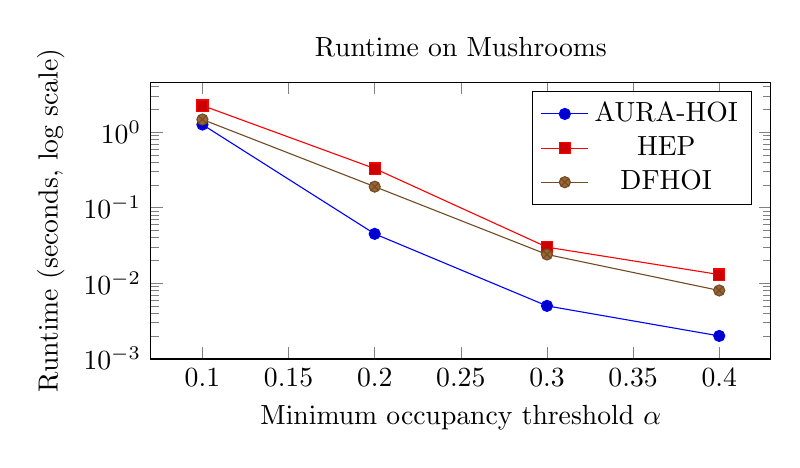
\begin{tikzpicture}
\begin{axis}[
  width=0.78\linewidth,
  height=0.42\linewidth,
  ymode=log,
  xlabel={Minimum occupancy threshold $\alpha$},
  ylabel={Runtime (seconds, log scale)},
  legend pos=north east,
  title={Runtime on Mushrooms}
]
\addplot coordinates {(0.10,1.262) (0.20,0.045) (0.30,0.005) (0.40,0.002)};
\addlegendentry{AURA-HOI}
\addplot coordinates {(0.10,2.256) (0.20,0.330) (0.30,0.030) (0.40,0.013)};
\addlegendentry{HEP}
\addplot coordinates {(0.10,1.474) (0.20,0.190) (0.30,0.024) (0.40,0.008)};
\addlegendentry{DFHOI}
\end{axis}
\end{tikzpicture}
\caption{Runtime under raw fullset output and matched summed-occupancy semantics.}
\label{fig:runtime}
\end{figure}

\begin{figure}[t]
\centering
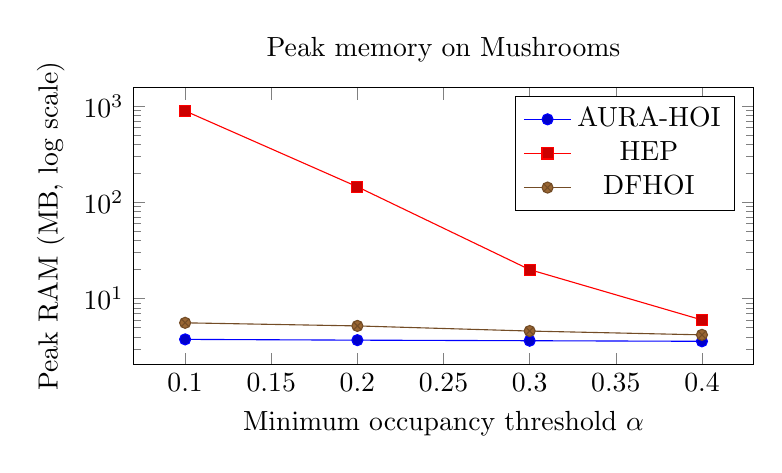
\begin{tikzpicture}
\begin{axis}[
  width=0.78\linewidth,
  height=0.42\linewidth,
  ymode=log,
  xlabel={Minimum occupancy threshold $\alpha$},
  ylabel={Peak RAM (MB, log scale)},
  legend pos=north east,
  title={Peak memory on Mushrooms}
]
\addplot coordinates {(0.10,3.77) (0.20,3.70) (0.30,3.65) (0.40,3.60)};
\addlegendentry{AURA-HOI}
\addplot coordinates {(0.10,890.74) (0.20,145.0) (0.30,20.0) (0.40,6.0)};
\addlegendentry{HEP}
\addplot coordinates {(0.10,5.60) (0.20,5.20) (0.30,4.60) (0.40,4.20)};
\addlegendentry{DFHOI}
\end{axis}
\end{tikzpicture}
\caption{Peak resident memory. The main advantage appears at low thresholds where candidate-heavy methods materialize substantially more intermediate evidence.}
\label{fig:memory}
\end{figure}

\subsection{Ablation plan}
Ablation is required to determine which design components matter. Table~\ref{tab:ablation} lists the intended variants. The current draft reports the design of the ablation; final submission should include measured runtime, memory, visited nodes, and itemset counts for each variant.

\begin{table}[t]
\centering
\small
\caption{Ablation variants for isolating AURA-HOI components.}
\label{tab:ablation}
\begin{tabular}{p{0.25\linewidth}p{0.25\linewidth}p{0.40\linewidth}}
\toprule
Variant & Removed component & Expected effect \\
\midrule
AURA-HOI-Full & none & Best balance of correctness, runtime, memory, and auditability. \\
AURA-HOI-noLedger & support-class ledger & Duplicate support classes may reappear; closed-output validation becomes weaker. \\
AURA-HOI-noResidual & residual envelope & More visited nodes, especially at medium and high occupancy thresholds. \\
AURA-HOI-noClosure & closure jumping & Deeper DFS traversal and larger representative output. \\
AURA-HOI-rawOnly & closed output disabled & Correct raw output but no compact support-class view. \\
AURA-HOI-heapMemory & arena or contiguous temporaries replaced by heap allocation & Higher allocation overhead and potentially higher peak RSS. \\
\bottomrule
\end{tabular}
\end{table}

\section{Discussion}
\subsection{Interpretation of the results}
The current results support two claims. First, AURA-HOI can match HEP and DFHOI under raw summed-occupancy semantics, which is necessary before comparing efficiency. Second, under this equal-output condition, AURA-HOI reduces memory substantially against HEP on Mushrooms at $\alpha=0.10$. This suggests that the combination of vertical evidence, pruning, and reduced candidate materialization can improve systems behavior without changing the raw output set.

The results should be interpreted conservatively. The strongest memory advantage appears on the dense Mushrooms setting, where HEP's level-wise candidate materialization is expensive. Retail has fewer emitted itemsets at the tested thresholds, so all algorithms have small absolute runtimes and memory usage. More datasets and thresholds are needed before making broad claims about dominance across all transactional data profiles.

\subsection{Threats to validity}
There are four main threats to validity. First, output semantics must remain matched. If one algorithm emits raw itemsets and another emits closed representatives, runtime and count comparisons are not meaningful. Second, the compatibility mode must be documented clearly because summed occupancy and average occupancy are different predicates. Third, benchmark results should be regenerated from scripts and CSV files rather than manually copied into the paper. Fourth, the implementation should include an independent checker that recomputes support, occupancy, closure, and support-bitset hashes from the original dataset.

\subsection{Limitations and future work}
AURA-HOI currently focuses on HOI-only mining. It does not handle utility, profit, sequence, temporal, or shelf-time information. The closed-ledger view is useful for compact analysis, but it should not be presented as a replacement for raw output in settings where all threshold-satisfying itemsets are required. Future work should extend the benchmark matrix, include additional public datasets, implement the ablation study, and evaluate top-$k$ behavior under the same audit framework.

\subsection{Reproducibility protocol}
A reproducible artifact should include the source code, dataset preprocessing scripts, benchmark driver, result CSV files, and figure-generation scripts. Each result row should contain the dataset, algorithm, support threshold, occupancy threshold, output view, runtime, peak RSS, disk estimate, emitted itemsets, and correctness hash. Pattern contents should be written only when correctness checking is explicitly requested; normal benchmark runs should output statistics by default.

\bibliographystyle{plain}
\begin{thebibliography}{99}

\bibitem{agrawal1993mining}
Rakesh Agrawal, Tomasz Imieli\'nski, and Arun Swami.
\newblock Mining association rules between sets of items in large databases.
\newblock In \emph{Proceedings of the 1993 ACM SIGMOD International Conference on Management of Data}, pages 207--216, 1993.
\newblock doi:10.1145/170035.170072.

\bibitem{agrawal1994fast}
Rakesh Agrawal and Ramakrishnan Srikant.
\newblock Fast algorithms for mining association rules in large databases.
\newblock In \emph{Proceedings of the 20th International Conference on Very Large Data Bases}, pages 487--499, 1994.

\bibitem{deng2020mining}
Zhi-Hong Deng.
\newblock Mining high occupancy itemsets.
\newblock \emph{Future Generation Computer Systems}, 102:222--229, 2020.
\newblock doi:10.1016/j.future.2019.07.039.

\bibitem{han2000mining}
Jiawei Han, Jian Pei, and Yiwen Yin.
\newblock Mining frequent patterns without candidate generation.
\newblock In \emph{Proceedings of the 2000 ACM SIGMOD International Conference on Management of Data}, pages 1--12, 2000.
\newblock doi:10.1145/335191.335372.

\bibitem{kim2022mining}
Hyoju Kim, Taehyung Ryu, Changhoon Lee, Hyunmin Kim, Truong Truong, Philippe Fournier-Viger, Witold Pedrycz, and Unil Yun.
\newblock Mining high occupancy patterns to analyze incremental data in intelligent systems.
\newblock \emph{ISA Transactions}, 131:460--475, 2022.

\bibitem{luna2019review}
Jos\'e Mar\'ia Luna, Ramesh Uday Kiran, Philippe Fournier-Viger, and Sebasti\'an Ventura.
\newblock Frequent itemset mining: A 25 years review.
\newblock \emph{Wiley Interdisciplinary Reviews: Data Mining and Knowledge Discovery}, 9(6):e1329, 2019.
\newblock doi:10.1002/widm.1329.

\bibitem{nguyen2023efficient}
Linh T. T. Nguyen, Thanh Mai, Gia-Han Pham, Unil Yun, and Bay Vo.
\newblock An efficient method for mining high occupancy itemsets based on equivalence class and early pruning.
\newblock \emph{Knowledge-Based Systems}, 267:110441, 2023.

\bibitem{pasquier1999discovering}
Nicolas Pasquier, Yves Bastide, Rafik Taouil, and Lotfi Lakhal.
\newblock Discovering frequent closed itemsets for association rules.
\newblock In \emph{Proceedings of the 7th International Conference on Database Theory}, pages 398--416, 1999.
\newblock doi:10.1007/3-540-49257-7\_25.

\bibitem{yildirim2025topk}
\.Irfan Y\i ld\i r\i m.
\newblock Mining top-k high occupancy itemsets.
\newblock \emph{Black Sea Journal of Engineering and Science}, 8(6):1723--1730, 2025.
\newblock doi:10.34248/bsengineering.1744061.

\bibitem{zaki1997new}
Mohammed J. Zaki, Srinivasan Parthasarathy, Mitsunori Ogihara, and Wei Li.
\newblock New algorithms for fast discovery of association rules.
\newblock In \emph{Proceedings of the Third International Conference on Knowledge Discovery and Data Mining}, pages 283--286, 1997.

\bibitem{zaki2000scalable}
Mohammed J. Zaki.
\newblock Scalable algorithms for association mining.
\newblock \emph{IEEE Transactions on Knowledge and Data Engineering}, 12(3):372--390, 2000.
\newblock doi:10.1109/69.846291.

\bibitem{zaki2002charm}
Mohammed J. Zaki and Ching-Jiu Hsiao.
\newblock CHARM: An efficient algorithm for closed itemset mining.
\newblock In \emph{Proceedings of the Second SIAM International Conference on Data Mining Workshop on High Performance Data Mining}, 2002.

\end{thebibliography}

\end{document}